\documentclass{article}

\usepackage{common}

\title{ecma-llvm compile process}
\author{KokaKiwi}
\date{}

\makeindex

\begin{document}

    \maketitle

    \begin{abstract}

        This document describes the ecma-llvm compile-process.

    \end{abstract}

    \newpage
    \tableofcontents

    \newpage
    \section{Diagram}

        \begin{center}
            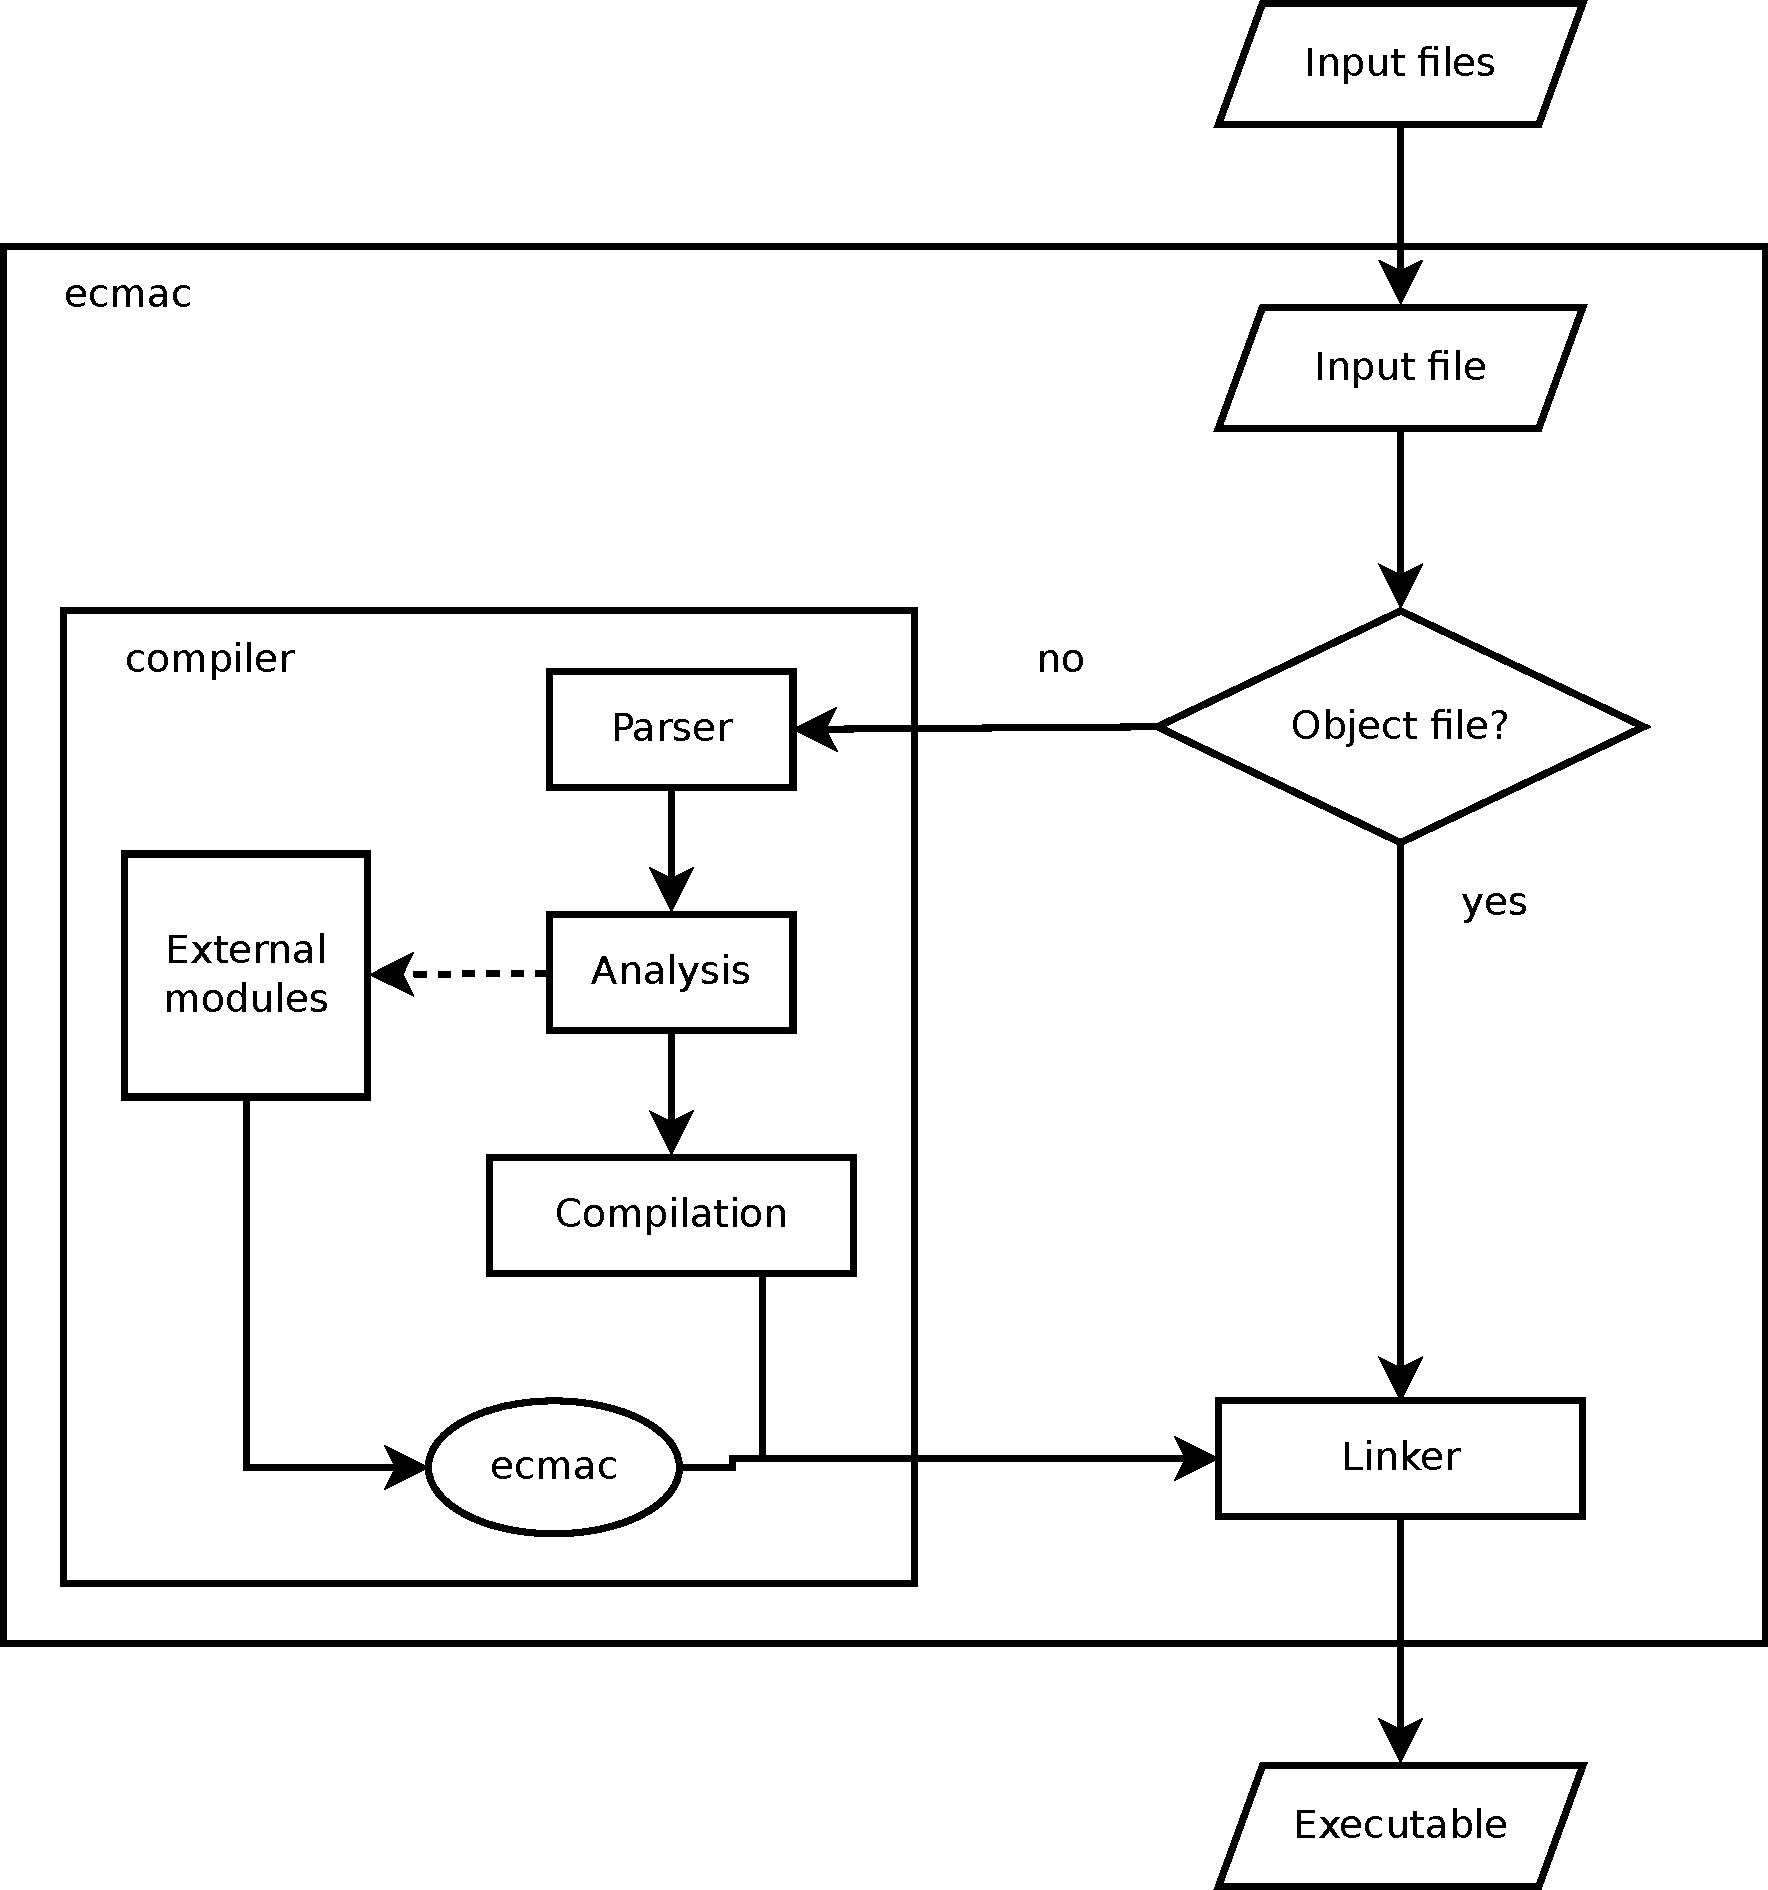
\includegraphics[width=16cm]{compile-flow-diagram.pdf}
        \end{center}

    \newpage
    \section{Compilation process}

        \subsection{Frontend}

            The frontend is the main interface of the compiler: ecmac

            It accepts any number of arguments and options.

            Each positionnal arguments are considered as input files.

            For each input file, the frontend test if it's an object file (or an up-to-date existing object file for this input file).

            \begin{notice}
                Use flag \emph{-P} or \emph{--parse-only} to stop compiler at parse-time.
            \end{notice}

    \newpage
    \printindex

\end{document}
